\documentclass[border=10pt]{standalone}
\usepackage{fontspec}\usepackage{tikz}
\usetikzlibrary{arrows.meta,positioning}
\definecolor{NouOrange}{HTML}{FA4D1F}\definecolor{NouBlack}{HTML}{000000}
\begin{document}
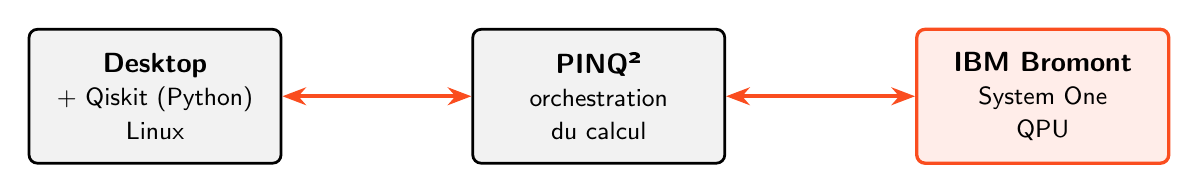
\begin{tikzpicture}[font=\sffamily,
  b/.style={draw=NouBlack,line width=1pt,rounded corners=3pt,align=center,minimum width=3.2cm,minimum height=1.7cm,fill=black!5}]
  \node[b] (d) {\textbf{Desktop}\\{\small + Qiskit (Python)}\\{\small Linux}};
  \node[b,right=2.4cm of d] (p) {\textbf{PINQ²}\\{\small orchestration}\\{\small du calcul}};
  \node[b,right=2.4cm of p,draw=NouOrange,line width=1.2pt,fill=NouOrange!10] (ibm) {\textbf{IBM Bromont}\\{\small System One}\\{\small QPU}};
  \draw[{Stealth[length=3mm]}-{Stealth[length=3mm]},NouOrange,line width=1.4pt] (d) -- (p);
  \draw[{Stealth[length=3mm]}-{Stealth[length=3mm]},NouOrange,line width=1.4pt] (p) -- (ibm);
\end{tikzpicture}
\end{document}
